\subsection{Acetaldeide}

Abbiamo successivamente analizzato la molecola di acetaldeide
\begin{figure}[ht]
\begin{center}
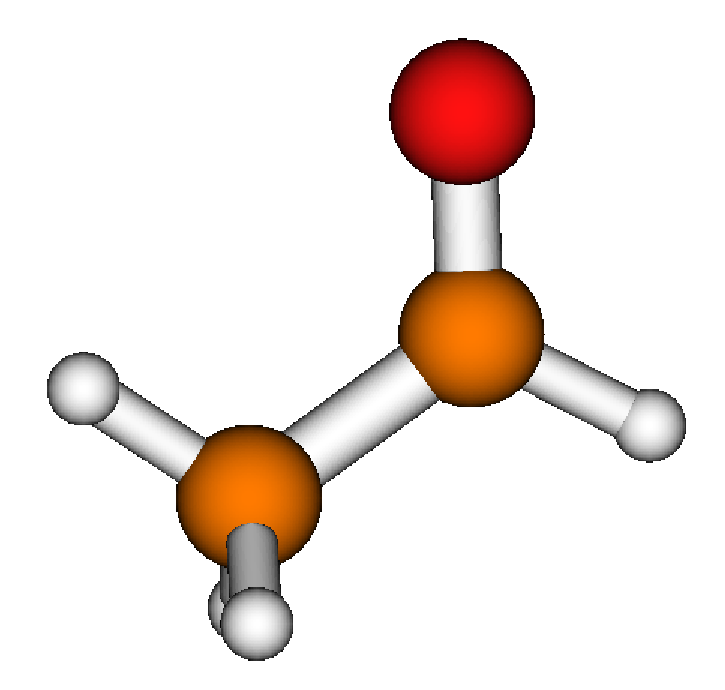
\includegraphics[angle=270,width=7cm,keepaspectratio]{immagini/acetaldeide/geom.eps}
\parbox[h]{10cm}{
\caption{\small Acetaldeide - configurazione spaziale per lo stato fondamentale}
\label{fig:acetaldeide_geom}
}
\end{center}
\end{figure}

Appartenente al gruppo C$_s$, l'acetaldeide ha presentato maggiori
difficolt\`a durante la trattazione richiesta, a causa della ridotta
simmetria rispetto alle molecole precedentemente analizzate. Tale
diversit\`a non consente un perfetto controllo della natura degli orbitali
che definiscono lo spazio CAS: la
selezione degli orbitali gi\`a descritta in precedenza deve ora appartenere
a due sole rappresentazioni irriducibili, la A$^{\prime}$ e la A$^{\prime\prime}$.

Nella tabella dei caratteri qui sotto riportata abbiamo posto l'asse $z$
allineato con il gruppo carbonile, ed il piano $yz$ come elemento di
simmetria per la riflessione \begin{center}
\begin{tabular}{c|cc|c}
  C$_s$				& E		& $\sigma_{yz}$	&           \\
\hline
    A$^{\prime}$  		& 1		&   1			&  $y$, $z$	\\
    A$^{\prime\prime}$	& 1		&  -1			&  $x$      \\
\end{tabular}
\end{center}
In questo modo, \`e possibile interpretare la molecola di acetaldeide, dal
punto di vista della simmetria, in maniera analoga alle molecole viste in
precedenza. Per questa ragione, gli orbitali $\pi$ e $\pistar$ apparterranno alla
rappresentazione irriducibile A$^{\prime\prime}$, in quanto antisimmetrici
rispetto alla riflessione sul piano della molecola, mentre i restanti
orbitali $n_y$, $\sigma$ e $\sigma^{*}$ apparterranno alla rappresentazione
A$^{\prime}$.

Al solito, si \`e scelto uno spazio attivo compatibile alle precedenti
caratterizzazioni e si sono effettuati calcoli sulla base 6-311G* al fine di
ottenere la geometria dello stato fondamentale. 
La scelta ha comportato uno spazio inattivo costituito da 8 orbitali di
simmetria A$^{\prime}$ e 1 orbitale di simmetria A$^{\prime\prime}$, e uno
spazio attivo di 3 orbitali A$^{\prime}$ e 2 orbitali A$^{\prime\prime}$.
Con questa scelta, per descrivere la molecola sono necessarie 28
configurazioni nell'espansione CAS-CI.

La figura \ref{fig:acetaldeide_orbitali_5} mostra gli orbitali dello spazio
attivo per lo stato fondamentale

\begin{figure}[htb]
\caption{\small Spazio CAS per l'acetaldeide}
\label{fig:acetaldeide_orbitali_5}
\begin{center}
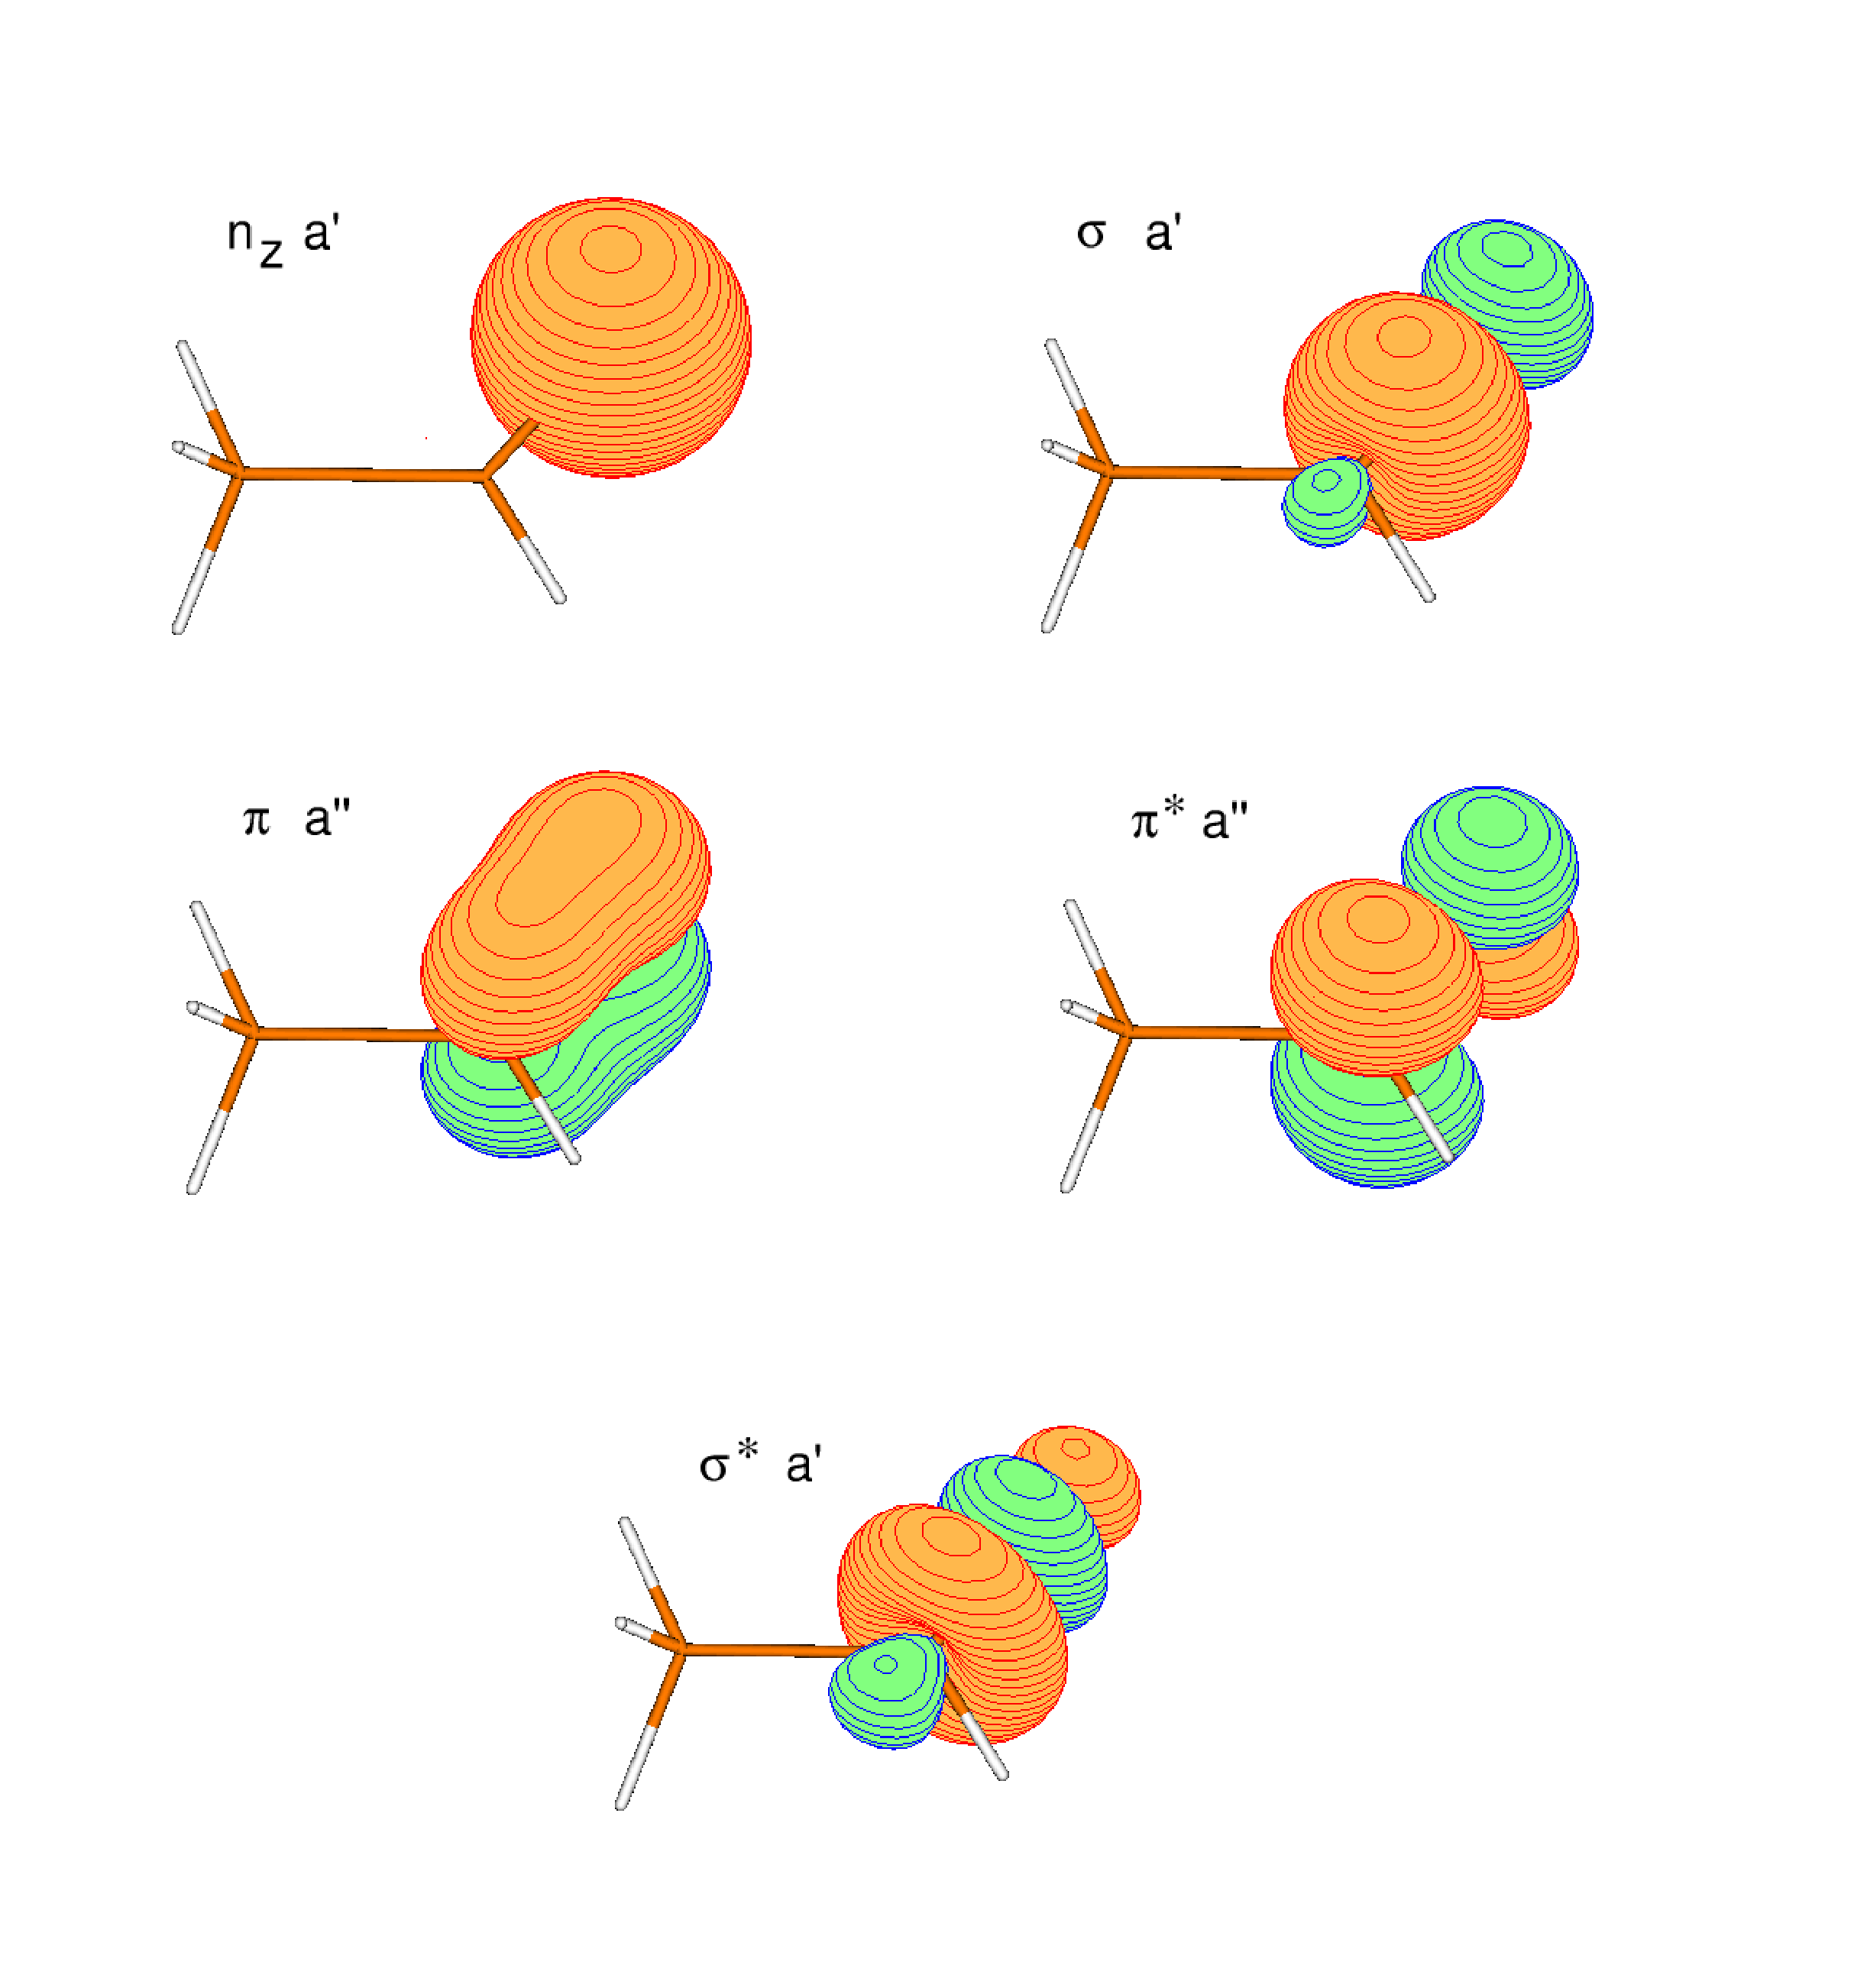
\includegraphics[width=9cm,keepaspectratio]{immagini/acetaldeide/orbitali_5.eps}
\end{center}
\end{figure}

\clearpage
Come \`e possibile notare, lo spazio attivo per lo stato fondamentale
\`e diverso da quello atteso: l'orbitale $n_y$ \`e stato
sostituito dall'orbitale $n_z$.

La ragione di tale variazione \`e imputabile al metodo di convergenza
dell'algoritmo CASSCF, che trova una migliore via di ottimizzazione (con
conseguente maggiore ottimizzazione variazionale dell'energia) attraverso
l'inclusione, nello spazio attivo, dell'orbitale $n_z$ anzich\'e dell'orbitale
$n_y$. Nei casi precedentemente trattati formaldeide e acetone, la simmetria
permetteva un controllo maggiore, in quanto gli orbitali $n_y$ ed $n_z$
appartenevano a rappresentazioni differenti.

Al contrario, lo stato eccitato di simmetria A$^{\prime\prime}$ ha il
corretto spazio attivo, in quanto il maggior contributo correlativo viene
ottenuto includendo gli orbitali interessati al fenomeno, e l'algoritmo
di ricerca del minimo energetico sceglie uno spazio fisicamente corretto.

Come conseguenza di tale errore, l'energia dello stato fondamentale \`e
troppo ottimizzata, perch\'e pi\`u bassa rispetto allo stato contenente
l'orbitale $n_y$ nello spazio attivo. Ne risulta perci\`o un'energia di
eccitazione sia verticale che adiabatica troppo alta.

Sebbene quindi uno spazio attivo cos\`i designato sia errato per questo tipo
di calcolo, la medesima strategia attuata su formaldeide e acetone \`e stata
attuata anche sull'acetaldeide, per meglio valutare come il metodo
perturbativo non sia in grado di porre rimedio ad una intrinseca incorretta
descrizione di uno degli stati di interesse. 
Seguir\`a uno studio ulteriore sulla molecola di
acetaldeide con uno spazio CAS allargato a 5 orbitali A$^{\prime}$ e 2
orbitali A$^{\prime\prime}$, che contenendo interamente la fisica di
interesse dovrebbe fornire, ed in effetti fornisce, risultati sensibilmente
pi\`u accurati.

L'ottimizzazione geometrica, riferita alla disposizione degli atomi mostrata
in figura, ha fornito i dati in tabella \ref{tab:acetaldeide_geom}

\begin{figure}[ht]
\begin{center}
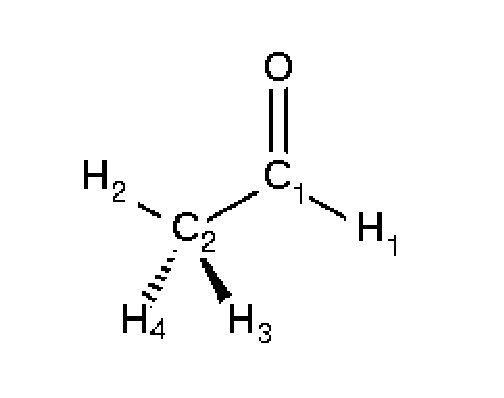
\includegraphics[angle=0,width=44mm,keepaspectratio]{immagini/acetaldeide/2d.eps}
\label{fig:acetaldeide_2d}
\end{center}
\end{figure}

\begin{center}
\begin{threeparttable}
\caption{\small Acetaldeide - geometria per lo stato fondamentale}
\label{tab:acetaldeide_geom}
\small
\begin{tabular}{|l|c|c|}
\hline
								& 6-311G*& Exp.\tnote{1} \\ %& 6-311G*/CAS $n_x \rightarrow \pistar$ \\
								& CAS(6,5)& 	 \\ %& 6-311G*/CAS $n_x \rightarrow \pistar$ \\
\hline
$r$(C$_1$-O)					& 1.21789		& 1.213 	\\%& 1.389869 \\
$r$(C$_1$-C$_2$)				& 1.50284		& 1.504		\\%& 1.497634 \\	
$r$(C$_1$-H$_1$)				& 1.09208		& 1.106		\\%& 1.078165 \\	
$r$(C$_2$-H$_2$)				& 1.08148		& 1.091		\\
$r$(C$_2$-H$_{3/4}$)			& 1.08588		& 1.085		\\
$\angle$(O-C$_1$-C$_2$)			& 124.007		& 124.0		\\%& 114.112 \\	
$\angle$(O-C$_1$-H$_1$)			& 119.395		& 121.1		\\%& 111.097 \\	
$\angle$(C$_2$-C$_1$-H$_1$)		& 116.598		& 114.9		\\%& 120.477 \\	
$\angle$(C$_1$-C$_2$-H$_{3/4}$)	& 110.148		& 110.6		\\%& 		 \\	
$\angle$(C$_1$-C$_2$-H$_2$)		& 110.347		& 110.6		\\%& 		 \\	
$\angle$(H$_3$-C$_2$-H$_4$)		& 107.232	 	&		\\%& 		 \\	
$\angle$(H$_2$-C$_2$-H$_{3/4}$)	& 109.454 		&		\\%& 		 \\	
$\tau$(O-C$_1$-C$_2$-H$_{3/4}$)	& $\pm120.959$	&		\\%& 		 \\	
\hline
\end{tabular}
\begin{tablenotes}
\small
 \item[1] Cfr. \cite{jpc-97-17-1993-4293}
 \item[] Distanze in Angstroms, angoli in gradi.
\end{tablenotes}
\end{threeparttable}
\end{center}

L'energia CASSCF a questa geometria \`e -153.024830 Hartree.
La transizione \mbox{$n_y \rightarrow \pistar$}, di simmetria $A^{\prime\prime}$,
ha energia CASSCF di -152.849283 Hartree. Conseguentemente, l'energia di transizione risulta essere 4.78 eV, contro
un valore sperimentale di 4.28 eV (Cfr. \cite{cpl-241-0-1995-26}).
Nel caso della transizione adiabatica, l'energia dello stato eccitato \`e -152.883379 Hartree, con una energia
di transizione pari a 3.85 eV, contro un valore sperimentale di 3.69 eV (Cfr. \cite{jpc-97-17-1993-4293})
La geometria di tale stato eccitato \`e mostrata in tabella \ref{tab:acetaldeide_geometrie_adiab}

\begin{center}
\begin{threeparttable}
\caption{\small Acetaldeide - geometria per lo stato eccitato adiabatico}
\label{tab:acetaldeide_geometrie_adiab}
\small
\begin{tabular}{|l|c|c|}
\hline
								& GS			&  $n_y \rightarrow \pistar$ \\ 
\hline
$r$($C_1$-O)					& 1.21789		& 1.38987 	\\
$r$($C_1$-$C_2$)				& 1.50284		& 1.49764	\\
$r$($C_1$-$H_1$)				& 1.09208		& 1.07816	\\
$r$($C_2$-$H_2$)				& 1.08148		& 1.08435	\\
$r$($C_2$-$H_3$)				& 1.08588		& 1.08290	\\
$r$($C_2$-$H_4$)				& 1.08588		& 1.08783	\\
$\angle$(O-$C_1$-$C_2$)			& 124.007		& 114.112	\\
$\angle$(O-$C_1$-$H_1$)			& 119.395		& 111.096	\\
$\angle$($C_1$-$C_2$-$H_1$)		& 116.598		& 120.478	\\
$\angle$($C_1$-$C_2$-$H_3$)		& 110.148		& 110.128	\\
$\angle$($C_1$-$C_2$-$H_4$)		& 110.148		& 111.455	\\
$\angle$($C_1$-$C_2$-$H_2$)		& 110.347		& 110.788   \\
$\angle$($H_3$-$C_2$-$H_4$)		& 107.232		& 108.365	\\
$\angle$($H_2$-$C_2$-$H_3$)		& 109.454		& 108.093	\\
$\angle$($H_2$-$C_2$-$H_4$)		& 109.454		& 107.902	\\
$\tau$(O-$C_1$-$C_2$-$H_4$)		& 120.959		&  65.135	\\
$\tau$(O-$C_1$-$C_2$-$H_3$)		& -120.959		& -174.562	\\
$\tau$(O-$C_1$-$C_2$-$H_2$)		& 0.0			& -55.029 	\\
$\tau$($H_2$-$C_2$-$C_1$-$H_1$)	& 180.0			& 168.836 	\\
\hline
\end{tabular}
\begin{tablenotes}
\small
 \item[] Distanze in Angstroms, angoli in gradi.
\end{tablenotes}
\end{threeparttable}
\end{center}
\subsubsection{Perturbazione su uno spazio CAS 6 elettroni/5 orbitali}

La tabella \ref{tab:acetaldeide_vertical_basis_5} presenta i risultati
ottenuti su un CAS con 6 elettroni in 5 orbitali, spazio CAS che, come gi\`a
enunciato, \`e errato in quanto descrive i due stati in modo sbilanciato.

\begin{center}
\begin{threeparttable}
\caption{\small Acetaldeide - Energia di transizione verticale {$n_y \rightarrow \pistar$} di singoletto, CAS 6 elettroni 5 orbitali}
\label{tab:acetaldeide_vertical_basis_5}
\small
\begin{tabular}{|c|ccc|ccc|}
\hline
Basis	& \multicolumn{3}{c|}{GS\tnote{1}}				& \multicolumn{3}{c|}{$n_y \rightarrow \pistar$ vert.\tnote{2}} \\
		& CASSCF		& NEV-PT	 	&	NEV-PT		& CASSCF		& NEV-PT	& NEV-PT  \\
		& 				& SC 			&	PC			& 				& SC		& PC 	 \\
\hline
6-31G	& 0.925561		& 1.143647		&	1.145329	& 4.19			& 4.07 		& 4.06	\\
cc-pVDZ	& 1.002377	 	& 1.380037		&	1.382306	& 4.74			& 4.49 		& 4.49	\\
ano-1	& 1.040915	 	& 1.415777		&	1.418769	& 4.74			& 4.51 		& 4.49	\\
6-311G*	& 1.024830	 	& 1.454798		&	1.457103	& 4.78			& 4.49 		& 4.50	\\
cc-pVTZ & 1.048304	 	& 1.568727		&	1.571395	& 4.78			& 4.48 		& 4.47	\\			
\hline
\hline
Exp.\tnote{3}&				& 				& 				& \multicolumn{3}{c|}{4.28} \\
\hline
\end{tabular}
\begin{tablenotes}
 \item[1] Energia come -(152 + valore) Hartree
 \item[2] Valori in eV
 \item[3] Cfr. \cite{jpc-97-17-1993-4293}
\end{tablenotes}
\end{threeparttable}
\end{center}

Come \`e possibile vedere, nonostante l'applicazione della trattazione
perturbativa, il risultato calcolato \`e ancora distante dal valore
sperimentale. Analogo risultato si ottiene dalla comparazione dei
valori per la transizione adiabatica

\begin{center}
\begin{threeparttable}
\caption{\small Acetaldeide - Energia di transizione adiabatica $n_y \rightarrow \pistar$ di singoletto, CAS 6 elettroni 5 orbitali}
\label{tab:acetaldeide_adiab_basis_5}
\small
\begin{tabular}{|c|ccc|ccc|}
\hline
Basis	& ZPE 			& ZPE 			& $\Delta$ZPE		& CASSCF	& NEV-PT			& NEV-PT  \\
		& 	(GS)		&  (Ecc.) 		& 					& ZPE		& SC/ZPE			& PC/ZPE  \\
\hline
6-31G	& 1.612			& 1.546			& -0.066			& 3.35			& 3.33			& 3.34 \\
cc-pVDZ & 1.593			& 1.534			& -0.059			& 3.78 			& 3.76			& 3.78 \\
ano-1	& 1.603			& 1.545			& -0.058			& 3.78			& 3.75 			& 3.77 \\
6-311G* & 1.600			& 1.545			& -0.055			& 3.79			& 3.78			& 3.80 \\
cc-pVTZ & 1.589			& 1.533			& -0.056			& 3.81			& 3.84			& 3.86 \\
\hline
\hline
Exp.\tnote{1}&				& 				& 					& \multicolumn{3}{c|}{3.69} \\
\hline
\end{tabular}
\begin{tablenotes}
 \item[1] Cfr. \cite{jpc-97-17-1993-4293}
 \item[ ] Valori in eV
\end{tablenotes}
\end{threeparttable}
\end{center}

Diagrammando le energie di transizione per questo caso, risulta ancora pi\`u
evidente come l'errore rispetto al dato sperimentale sia elevato, sia per la
transizione verticale che per quella adiabatica.

\begin{figure}[ht]
\begin{center}
\includegraphics[angle=270,width=10cm,keepaspectratio]{immagini/acetaldeide/energie_vert_5.eps} \\
\includegraphics[angle=270,width=10cm,keepaspectratio]{immagini/acetaldeide/energie_adiab_5.eps}
\parbox[h]{12cm}{
\caption{\small Acetaldeide - energia di transizione verticale (in alto) ed adiabatica (sopra) su basi differenti a livello CASSCF (linea rossa), NEV-PT/SC (linea verde) e NEV-PT/PC (linea blu) come funzione della base atomica.}
\label{fig:acetaldeide_energie_vert_5}
}
\end{center}
\end{figure}
\clearpage

\`E inoltre evidente come la trattazione perturbativa NEV-PT non riesca ad
effettuare una correzione significativa, in quanto lo scarto rispetto allo
sperimentale \`e causato da una differente natura fisica dello stato
fondamentale, sul quale la trattazione perturbativa non pu\`o recuperare.

